\section{Synthetic Instance Generation} \label{sec:instances}

To evaluate the proposed optimization model under controlled yet realistic operating conditions, synthetic instances were generated following statistical assumptions inspired by production behavior observed in mature conventional oilfields. The objective of this procedure is to reproduce key structural characteristics of real production systems while maintaining reproducibility and scalability.

For each well $i$, the maximum gross production $G_i$ (in $m^3/\text{day}$) is generated using a lognormal distribution. This choice reflects the empirical observation that well productivity in mature basins is strictly positive and typically exhibits right-skewed behavior, with a small number of high-performing wells and a majority of low-to-medium producers. Formally,

\[
G_i \sim \text{LogNormal}(\mu_G, \sigma_G),
\]

\noindent where parameters $\mu_G$ and $\sigma_G$ control the median production level and heterogeneity of the field, respectively. Increasing $\sigma_G$ produces instances with higher dispersion and greater optimization difficulty.


Net production $N_i$ is modeled as a fraction of gross production:
\[
N_i = \alpha_i G_i,
\]

\noindent where $\alpha_i \in (0,1)$ represents the effective recovery ratio. The parameter $\alpha_i$ is drawn from a Beta distribution:

\[
\alpha_i \sim \text{Beta}(a,b).
\]

The Beta distribution is selected due to its flexibility and bounded support. By choosing $a < b$, the distribution can be skewed toward lower values, representing high water-cut conditions commonly observed in mature conventional fields.


The initial regime $r_i \in (0,1)$ represents the current operating condition of each well relative to its maximum capacity. Since wells in conventional fields are typically operated near stable regimes rather than uniformly across the full range, $r_i$ is generated using a Beta distribution skewed toward higher values:

\[
r_i \sim \text{Beta}(a_r, b_r), \quad a_r > b_r.
\]

This assumption ensures concentration of regimes around moderate-to-high operational levels while allowing variability across wells.

Finally the operation risk and technical priority are computed as explained before to determine the cost of intervention in a certain well.

This approach ensures that the generated datasets capture structural properties of real production systems while allowing controlled experimental analysis.

\begin{figure}
    \centering
    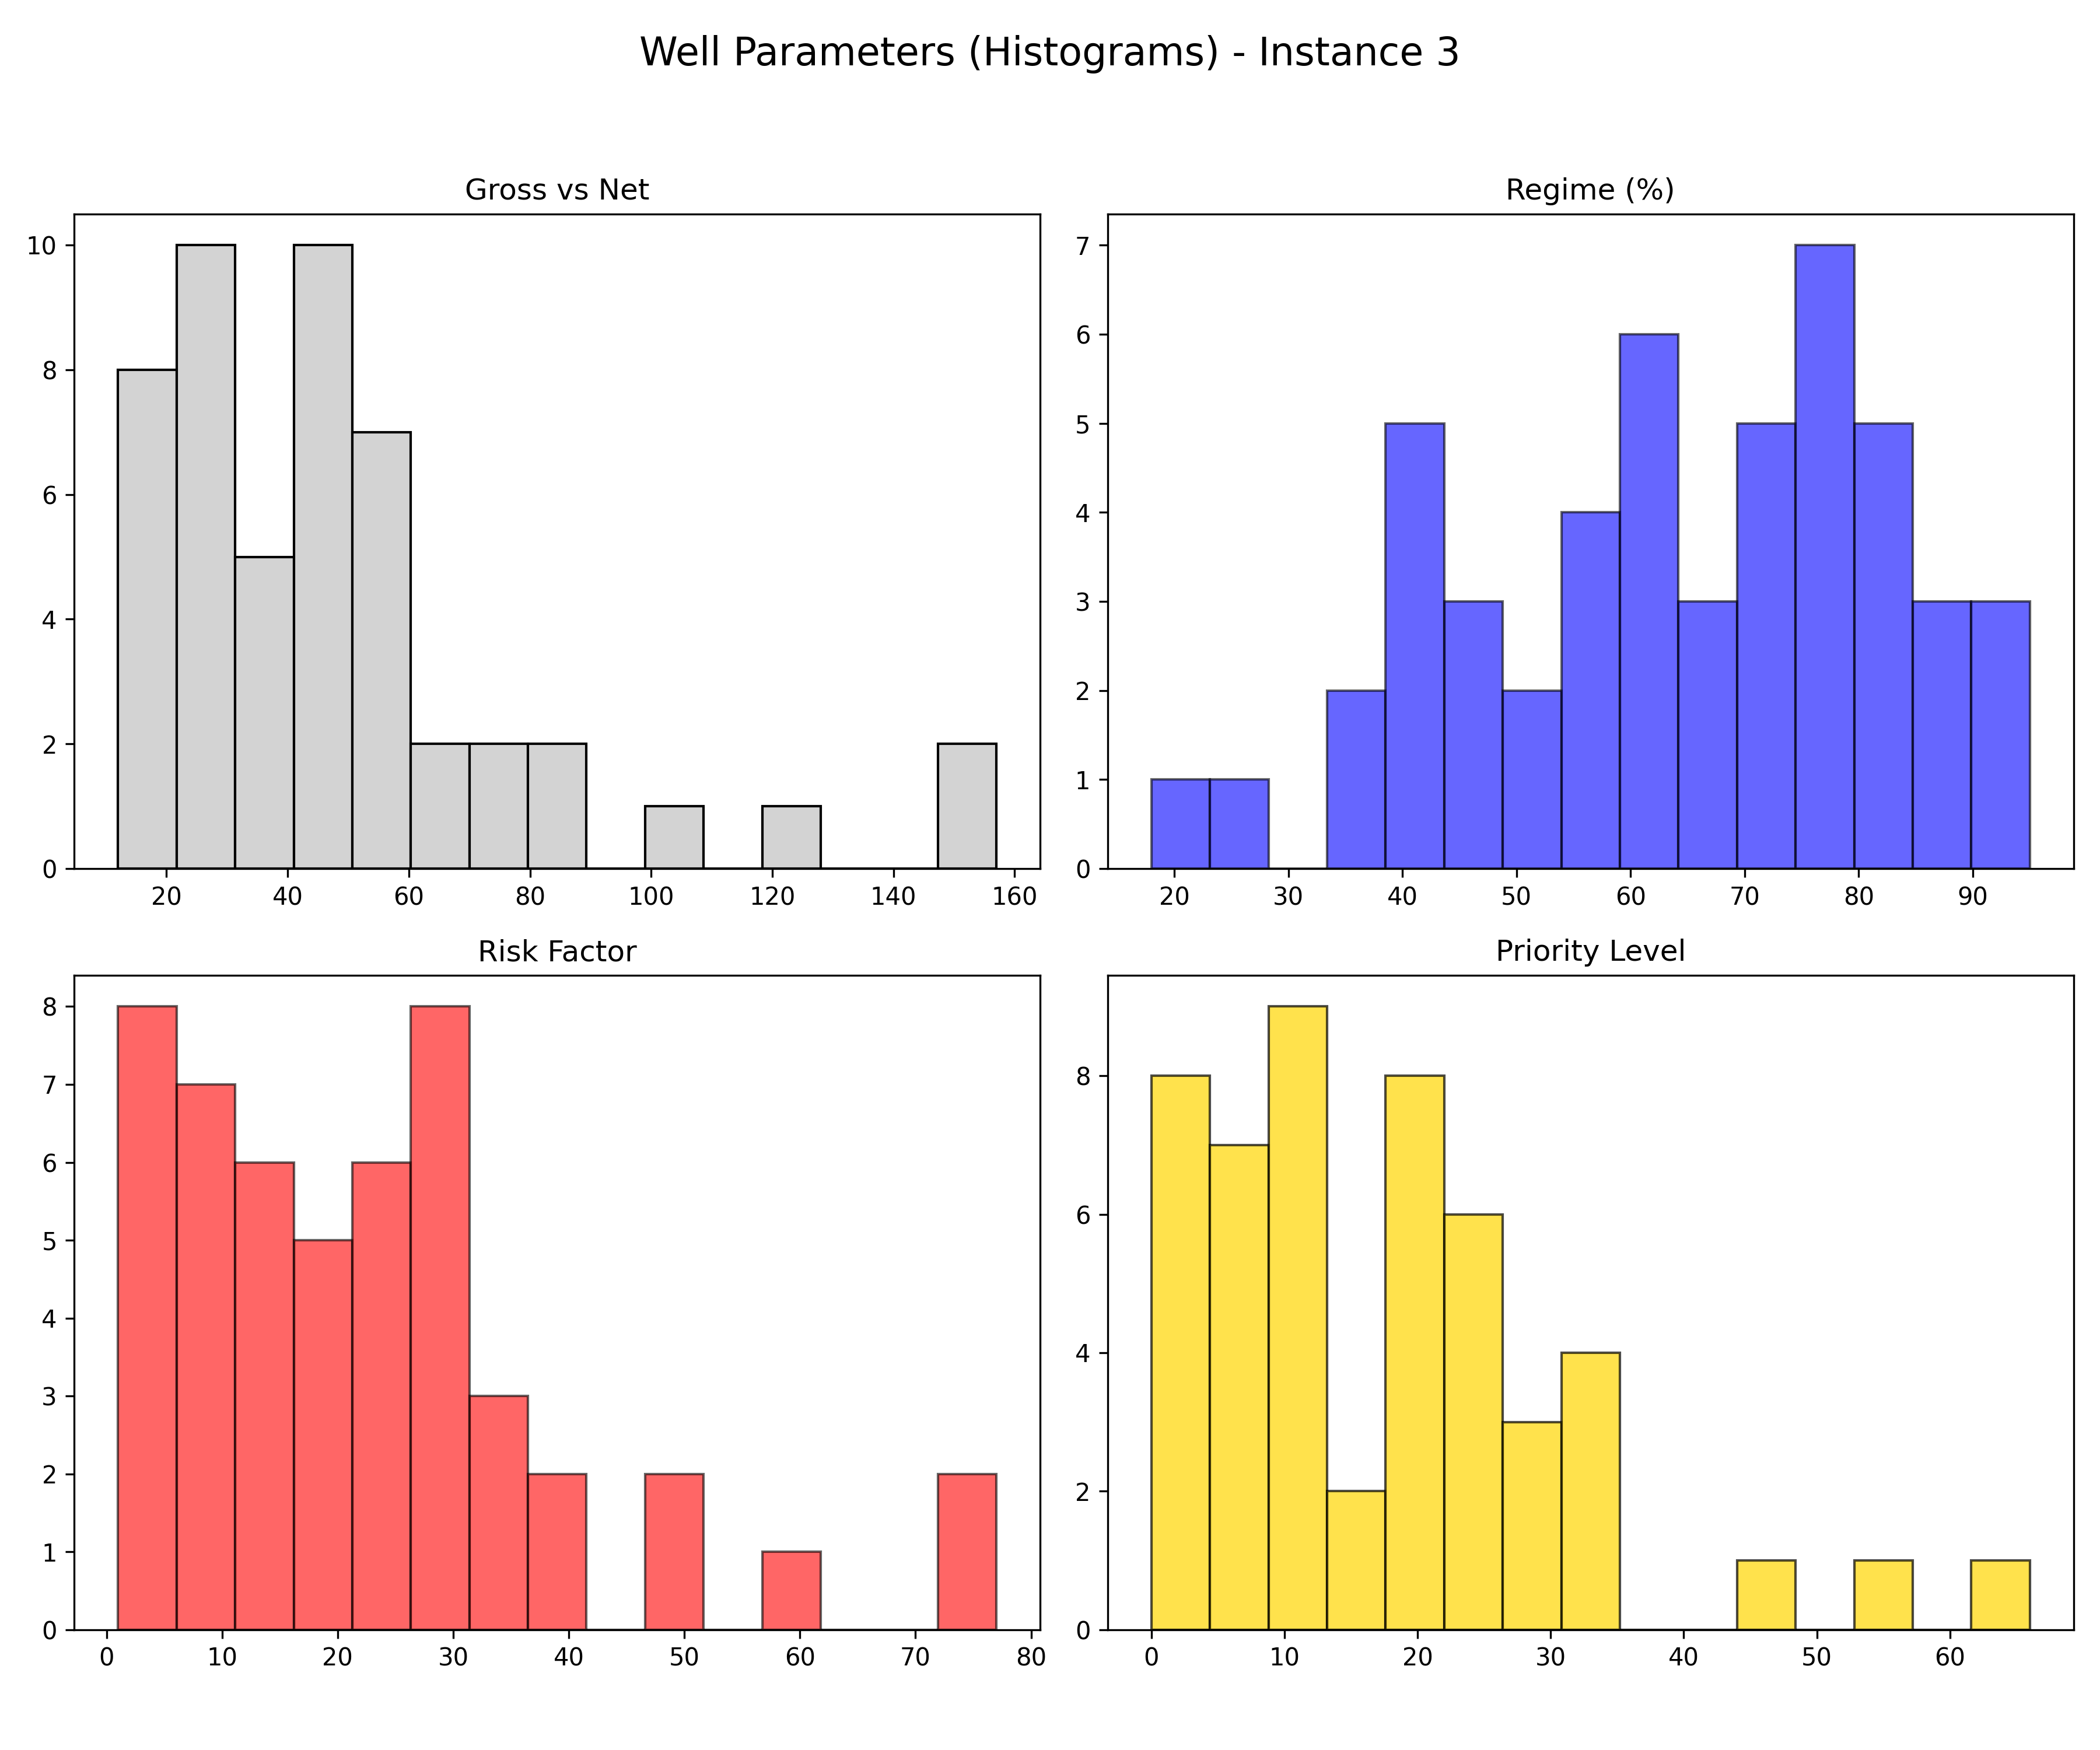
\includegraphics[width=0.75\textwidth]{imagenes/well_hist_1.png}
    \caption{Histograms of well parameters distribution}
    \label{fig:well_hist}
\end{figure}

\begin{figure}
    \centering
    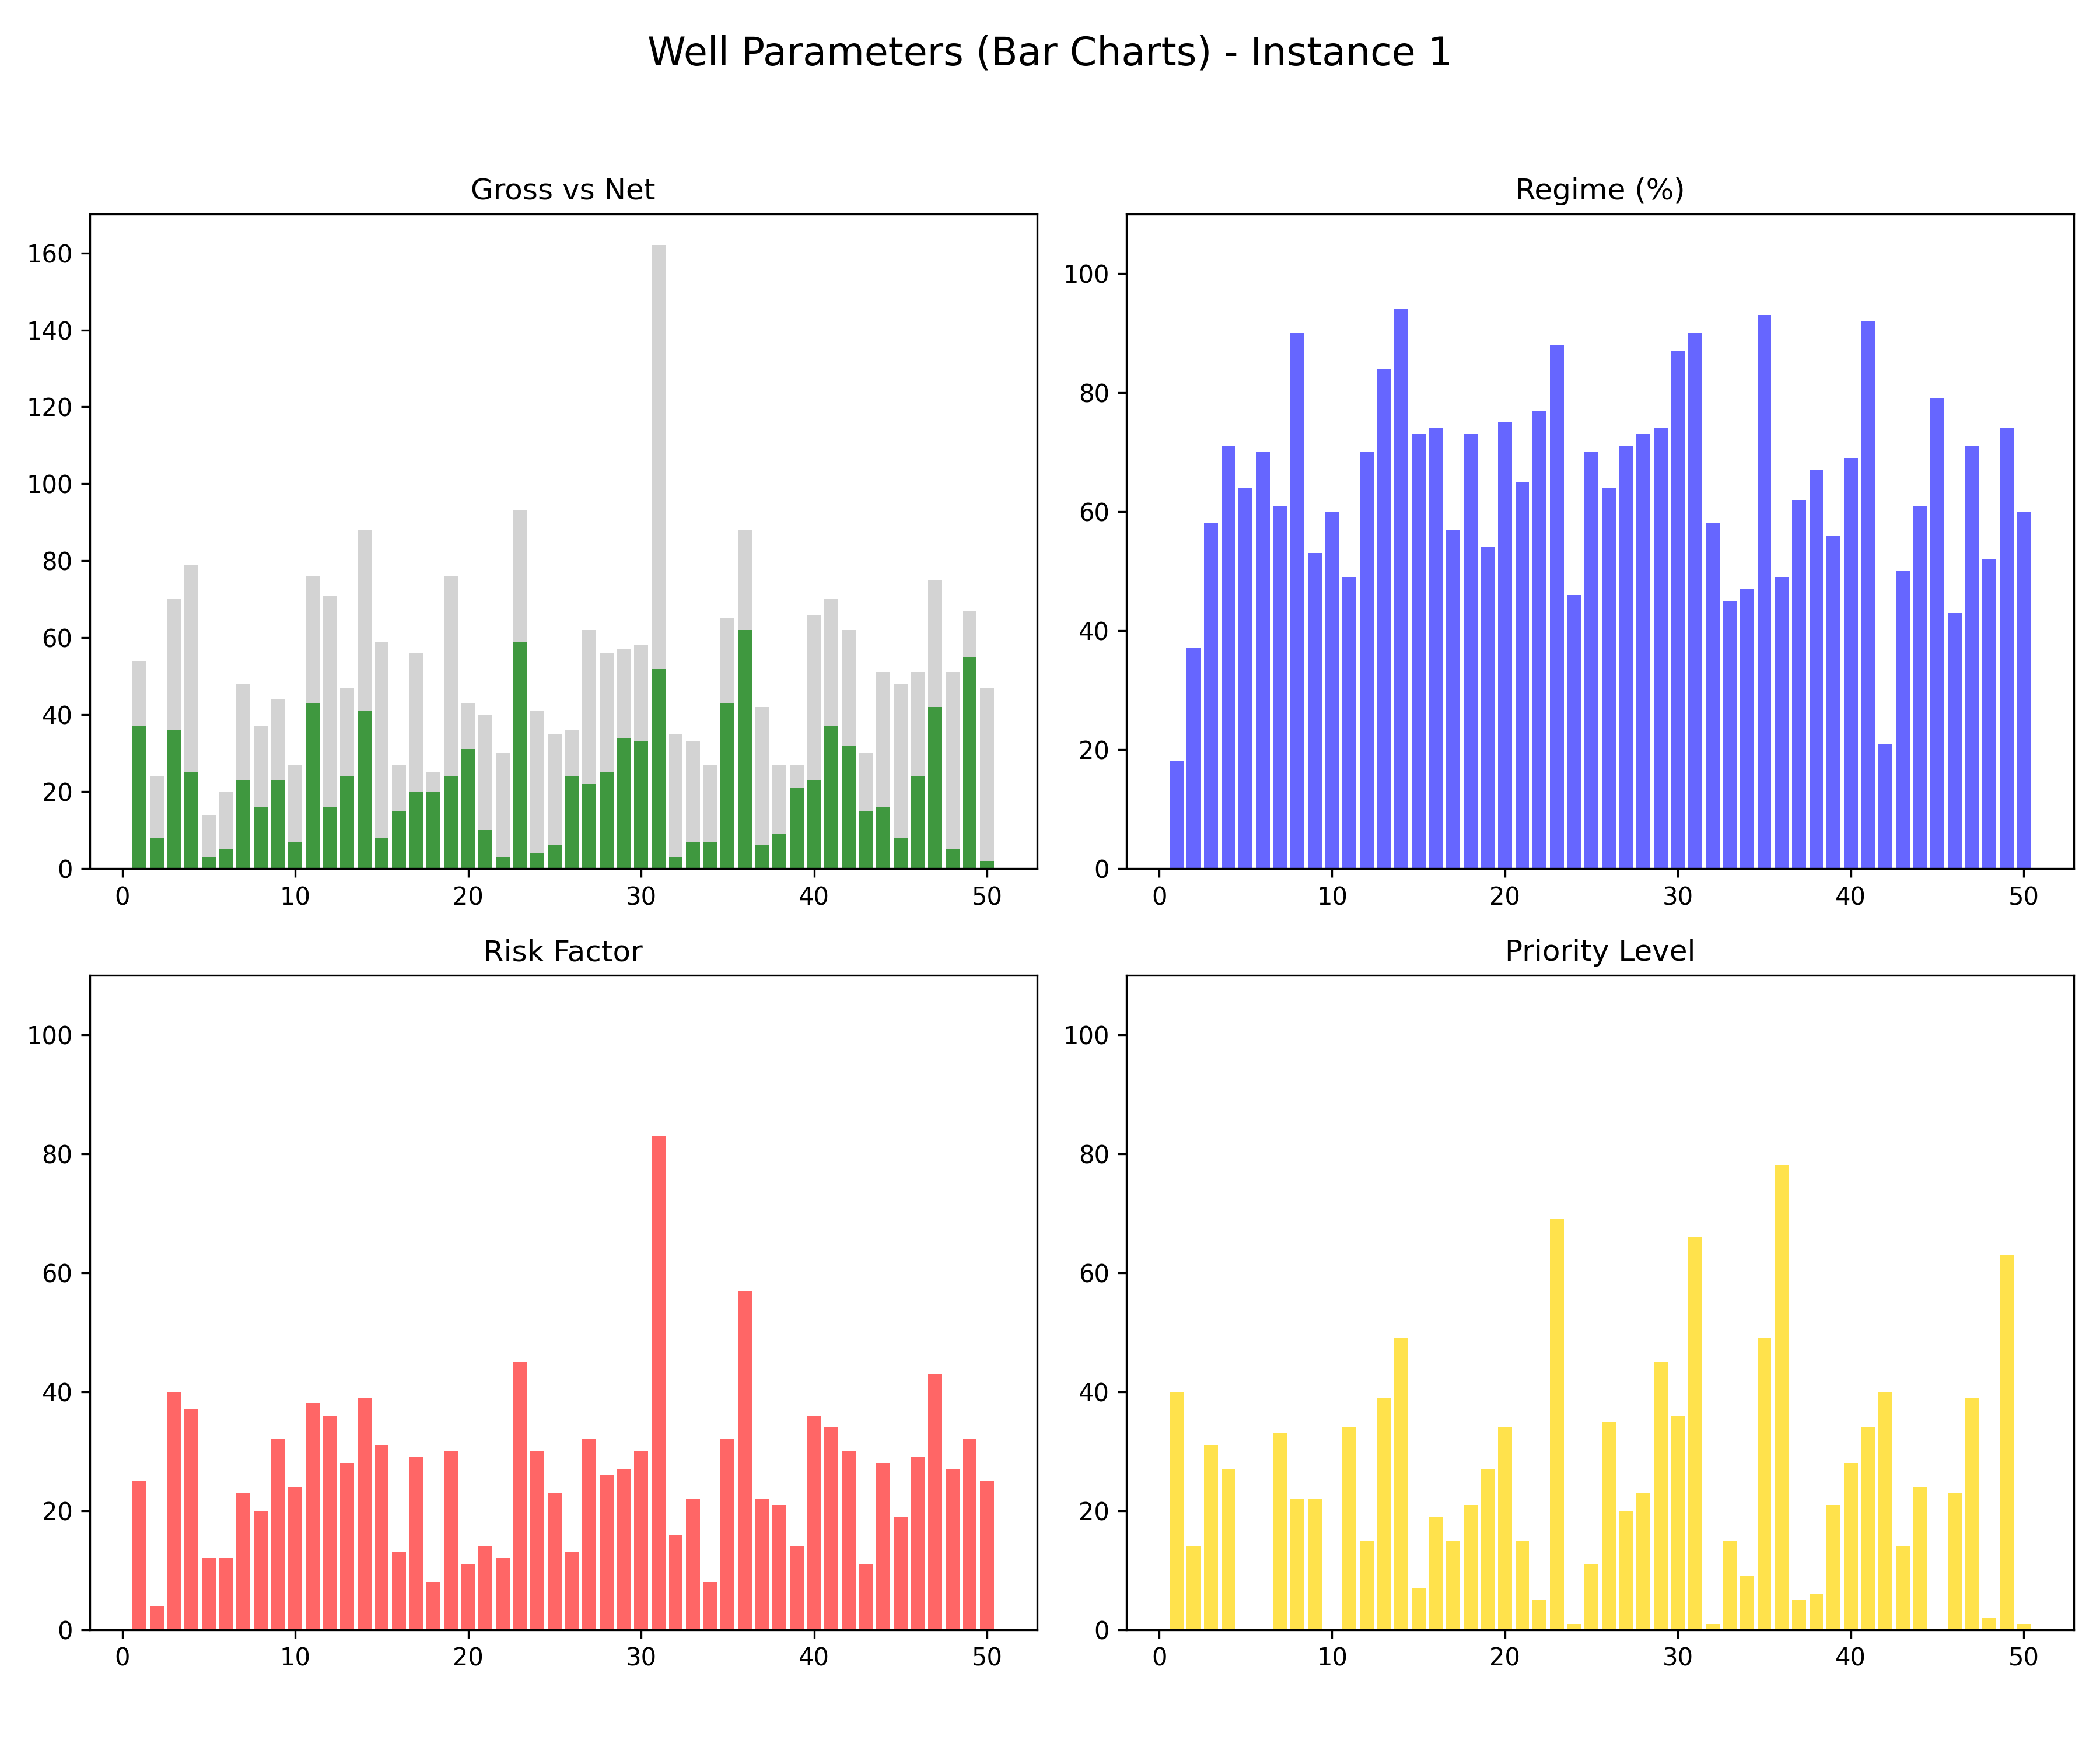
\includegraphics[width=0.75\textwidth]{imagenes/well_bar_1.png}
    \caption{Generated parameters of 50 wells sorted by ID}
    \label{fig:well_dist}
\end{figure}

To represent geographical dispersion and transportation effort in mature oilfields, a synthetic spatial environment is generated over a two-dimensional grid of size $L \times L$. Terrain elevation is produced by combining two components: (i) an interpolated low-resolution random field, and (ii) a configurable set of Gaussian peaks. Let $B(x,y)$ be the normalized interpolated base field and $P(x,y)$ the normalized peak field obtained from $n_{\text{peaks}}$ randomly centered Gaussian kernels. The final elevation is
\[
E(x,y) = A\,\big(\omega_b B(x,y) + \omega_p P(x,y)\big),
\]
where $A$ is the elevation amplitude, and $(\omega_b,\omega_p)=(0.35,0.65)$ in the current implementation. A Gaussian smoothing filter with parameter $\sigma_s$ is then applied. This design makes terrain ruggedness directly controllable through $n_{\text{peaks}}$, $A$, and $\sigma_s$.

Traversal difficulty is induced from topographic slope. Denoting by $\nabla E=(\partial_x E,\partial_y E)$ the discrete gradient (computed with Sobel operators), the slope magnitude is
\[
S(x,y)=\sqrt{(\partial_x E)^2+(\partial_y E)^2},
\]
and the movement cost map is defined as
\[
C(x,y)=1+S(x,y)^{\gamma},
\]
with exponent $\gamma$ controlling how strongly steep terrain is penalized.

Well locations are generated by sampling $n_{\text{clusters}}$ random cluster centers and drawing well coordinates from Gaussian clouds around each center, clipped to the grid domain. The operations center is placed near the geometric center of the field (within a bounded neighborhood) to emulate a central depot.

Road generation is performed in two stages using minimum accumulated-cost paths (MCP). First, primary roads connect each well to the operations center. After each path is created, traversed cells are assigned a very low dynamic cost, which encourages corridor reuse and creates realistic trunk-road consolidation. Second, secondary well-to-well connectors are added to induce loops and alternative routes. Candidate neighbor pairs are filtered by a maximum Euclidean radius and per-well degree limits. For each accepted pair, MCP is solved on a connector-specific map that penalizes reuse of primary-road cells; admissibility is enforced by comparing path cost against a scaled Euclidean threshold. This mechanism improves redundancy while avoiding degenerate overlap with the primary tree-like structure.

Finally, the distance matrix used in the MILP routing component is computed from terrain-based least-cost distances between all nodes (operations center plus wells). Therefore, transportation terms in the optimization model reflect anisotropic travel effort induced by terrain morphology, rather than simple Euclidean proximity.

\begin{figure}
    \centering
    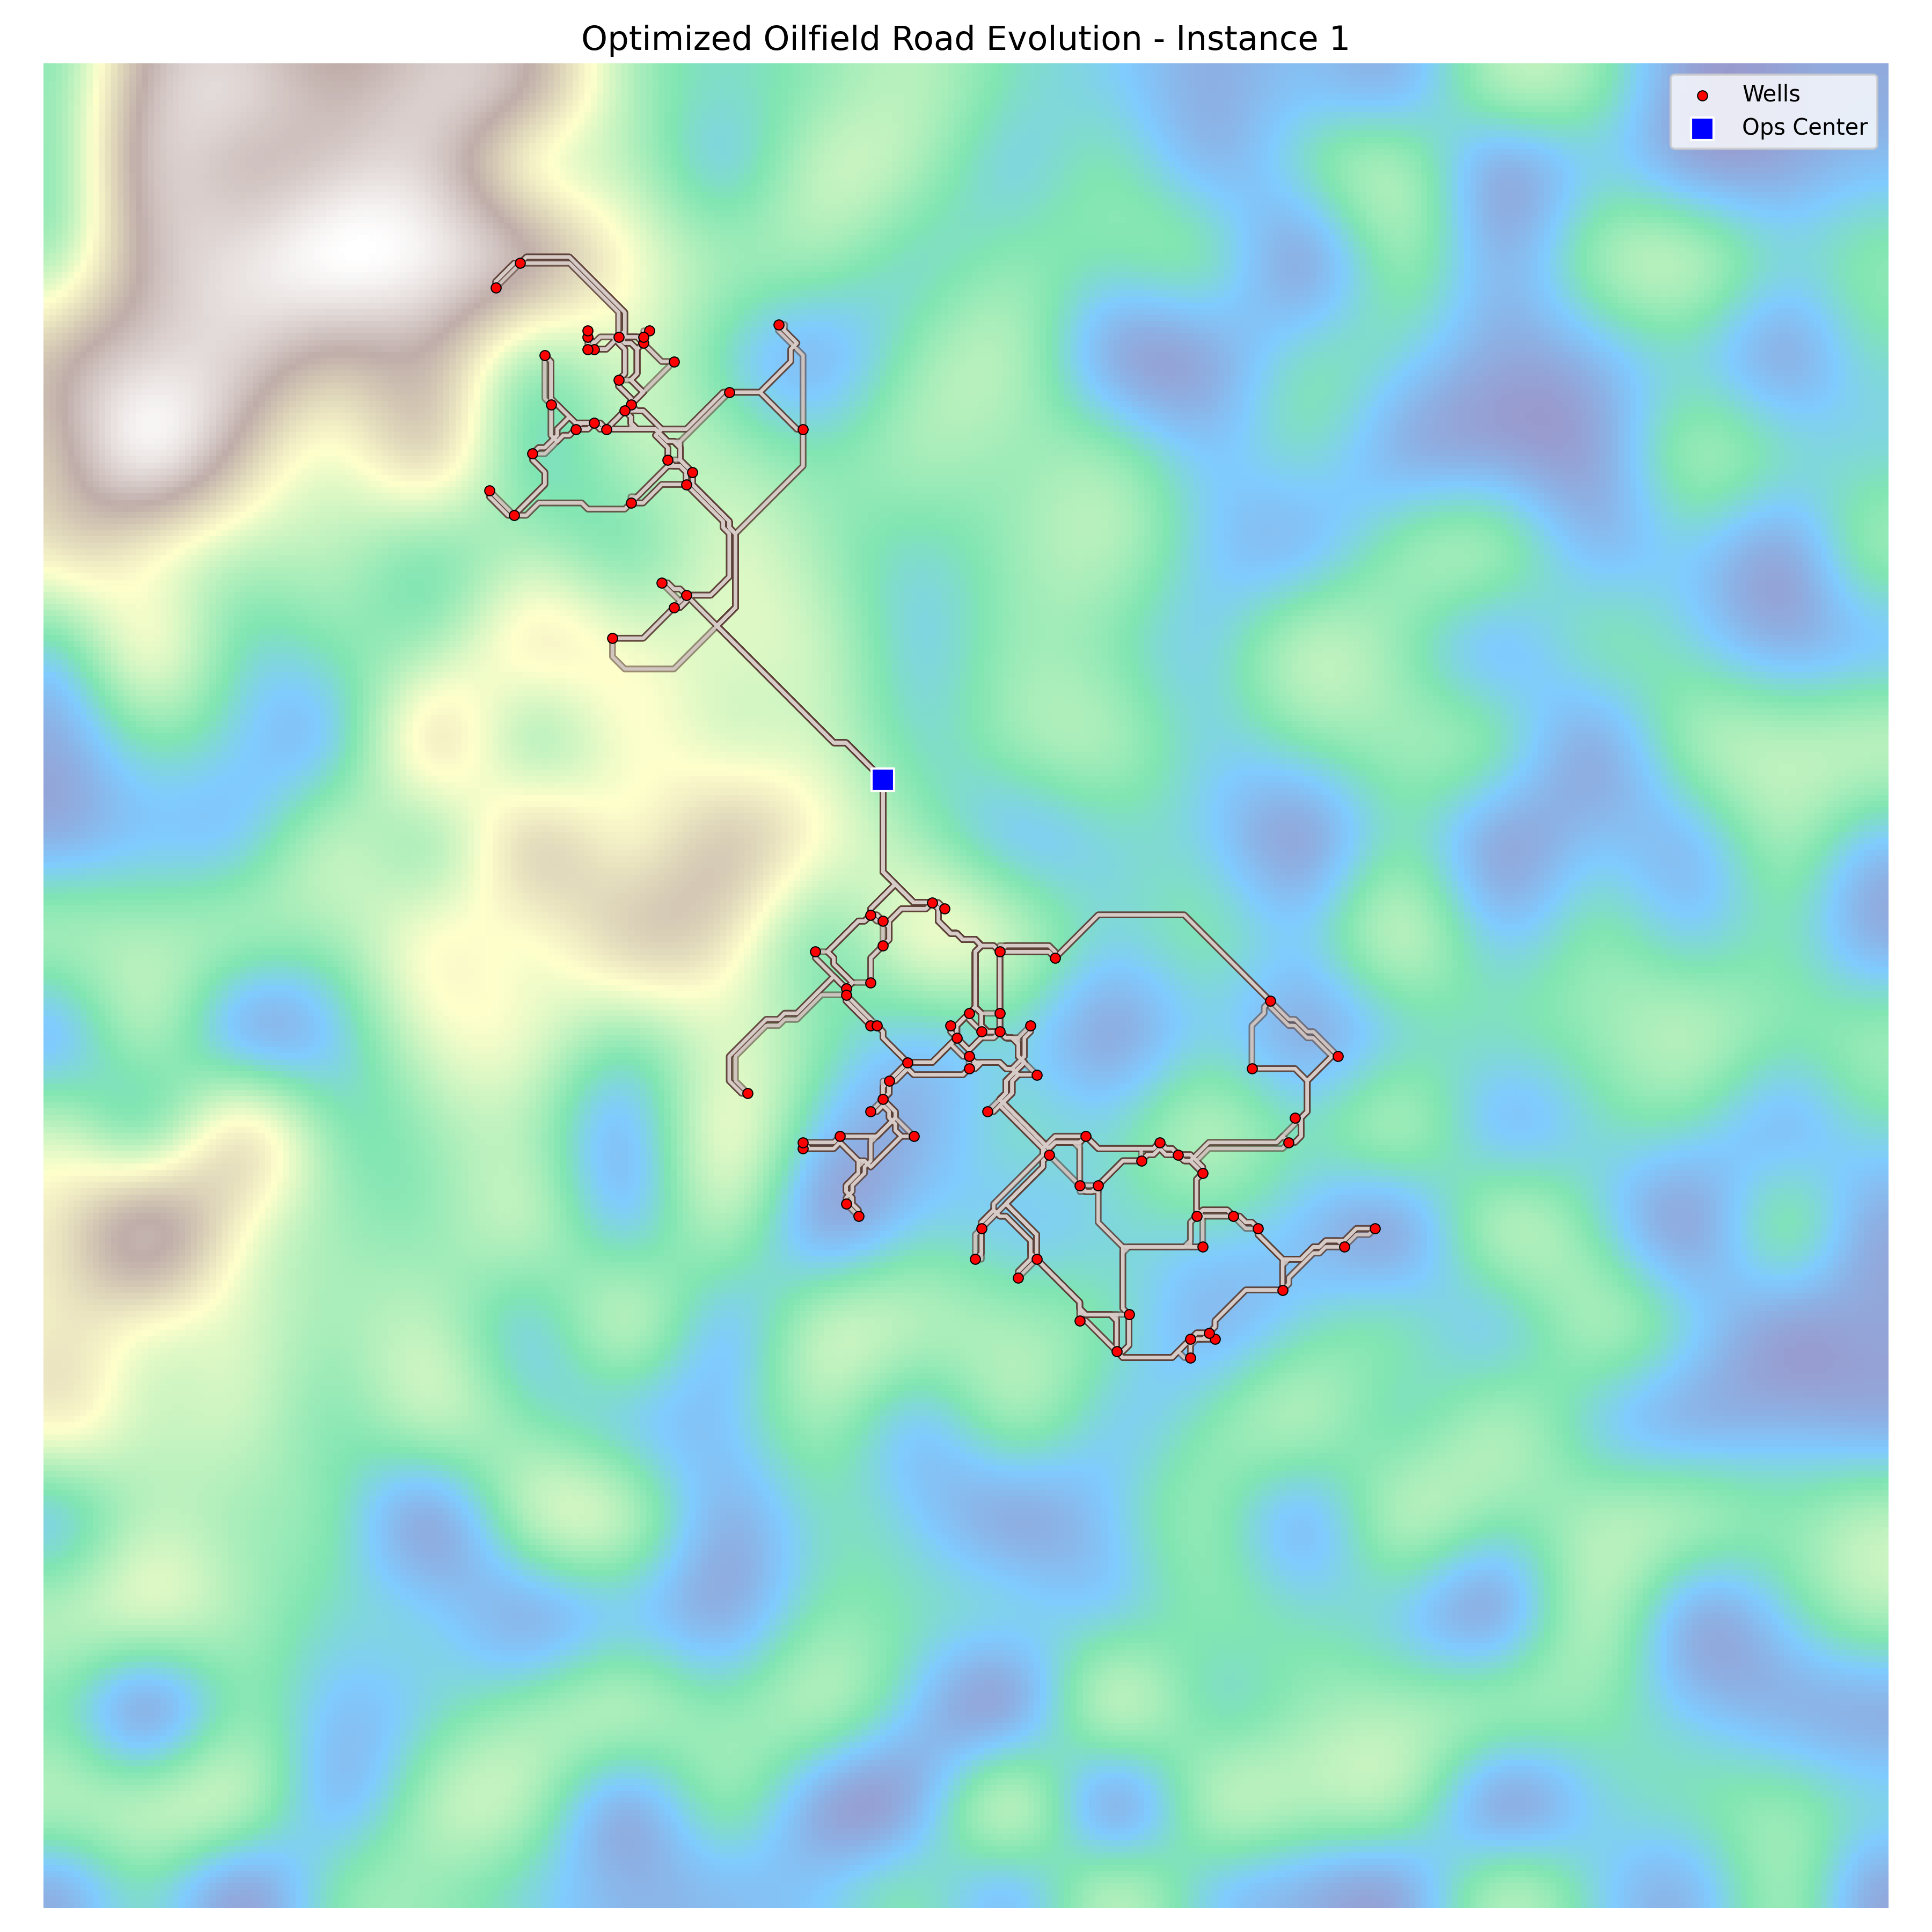
\includegraphics[width=0.75\textwidth]{imagenes/spatial_network_1.png}
    \caption{Procedural generated map of well locations and operations center}
    \label{fig:oil_field_map}
\end{figure}